\documentclass[11pt,a4paper]{article}
	% basic article document class
	% use percent signs to make comments to yourself -- they will not show up.

\usepackage{caption} %supress numbering figure from caption
\usepackage{hyperref}
\usepackage{tikz}
\usepackage{amsmath}
\usepackage{amssymb}
	% packages that allow mathematical formatting
\usepackage{float}
\usepackage{graphicx}
	% package that allows you to include graphics

\usepackage{setspace}
	% package that allows you to change spacing

\onehalfspacing
	% text become 1.5 spaced
\usepackage{wasysym} % contains the desired symbols

\usepackage{fullpage}
	% package that specifies normal margins

\usepackage{fancyhdr}
\pagestyle{fancy}
\lhead{Name: }
\rhead{                                                   }
%\lfoot{Lecture 1}
%\rfoot{Handout 1}




\setlength{\headheight}{14pt}

% Isocost lines (redrawn from Goolsbee et al., Microeconomics, 3e).
\definecolor{isogreen}{RGB}{0,166,118}
\newcommand{\isocostfigure}{%
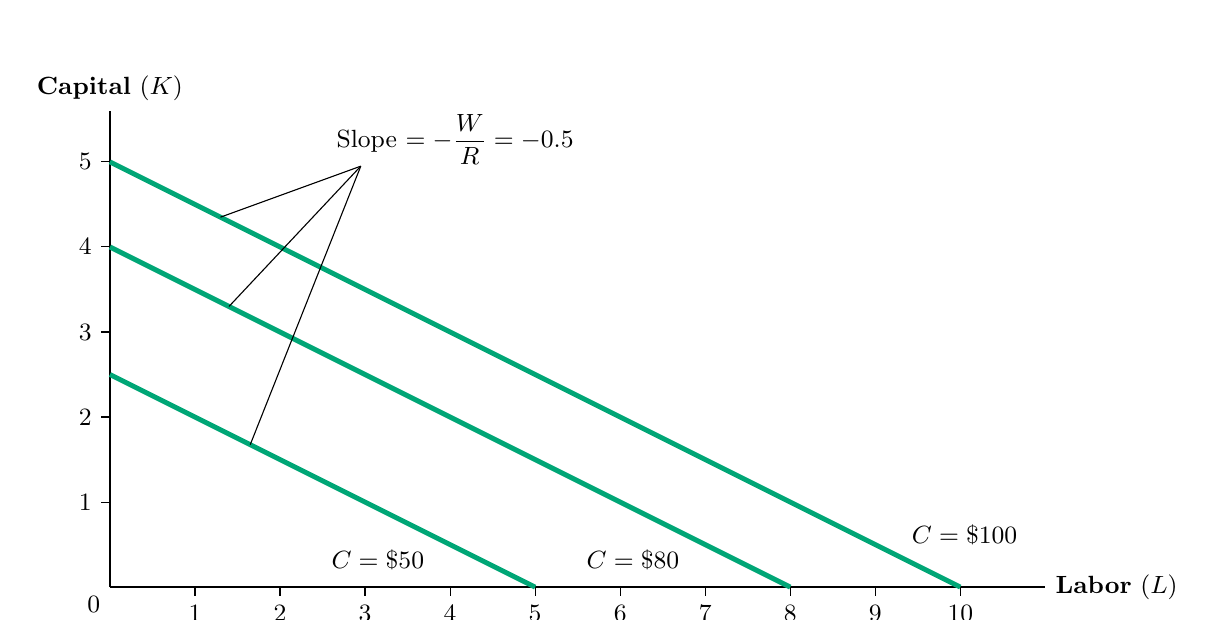
\begin{tikzpicture}[x=1.08cm,y=1.08cm,font=\small]
  % axes and ticks
  \foreach \x in {1,...,10} \draw (\x,0) -- (\x,-0.1) node[below] {\x};
  \foreach \y in {1,...,5} \draw (0,\y) -- (-0.1,\y) node[left] {\y};
  \node[below left] at (0,0) {0};
  \draw[thick] (0,0) -- (11,0) node[right] {\textbf{Labor} ($L$)};
  \draw[thick] (0,0) -- (0,5.6) node[above] {\textbf{Capital} ($K$)};
  % isocost lines
  \draw[line width=1.8pt,isogreen] (0,2.5) -- (5,0);
  \draw[line width=1.8pt,isogreen] (0,4) -- (8,0);
  \draw[line width=1.8pt,isogreen] (0,5) -- (10,0);
  \node at (3.15,0.32) {$C = \$50$};
  \node at (6.15,0.32) {$C = \$80$};
  \node at (10.05,0.62) {$C = \$100$};
  % slope label
  \node[anchor=south west] at (2.55,4.85) {Slope $= -\dfrac{W}{R} = -0.5$};
  \draw (2.95,4.95) -- (1.3,4.35);
  \draw (2.95,4.95) -- (1.4,3.3);
  \draw (2.95,4.95) -- (1.65,1.675);
\end{tikzpicture}}

\begin{document}
\title{Class 14 Quiz}
\author{PUBPOL 205}
\date{October 15, 2026}
\maketitle
\thispagestyle{fancy}
\begin{enumerate}
\item The graph below shows three isocost lines for a firm that hires labor ($L$) at wage $W$ and rents capital ($K$) at rental rate $R$. Is labor more expensive, or is capital more expensive? Why?
\begin{center}
\isocostfigure\\[2pt]
{\footnotesize Adapted from Goolsbee et al., \textit{Microeconomics}, 3e.}
\end{center}
\vfill
{
\bf (continued on the next page)}

\newpage
\thispagestyle{plain}
\item Consider a perfectly competitive firm in the short run. On the axes below, draw the firm's marginal cost ($MC$), average variable cost ($AVC$), and average total cost ($ATC$) curves, and sketch out the firm's short-run supply curve. Where is the break-even point? Where is the shutdown point? Label both on your graph.
\begin{center}
\begin{tikzpicture}[x=1.2cm,y=1.2cm,font=\small]
  \draw[thick,->] (0,0) -- (9.5,0) node[below left] {Quantity ($Q$)};
  \draw[thick,->] (0,0) -- (0,6.8) node[above] {Price, Cost (\$)};
  \node[below left] at (0,0) {0};
\end{tikzpicture}
\end{center}
\vfill
\end{enumerate}
\end{document}
